\chapter{State of the Art}


The research and interest in humanoid robotics has greatly increased over the last few years, but inspite of the current
abundance of the humanoid robots, their utility is still very limited. One of the most important trials, \textit{DARPA 
Robotics Challenge (DRC)} in 2013 listed a pack of capabilities and robustness that humanoid robots lacked when performing 
different tasks. Each task of this challenge should last only up to 30 minutes. These tasks will take less than a minute 
for a human to complete which  explains the powerlessness of the robots. This chapter briefly explains different control 
strategies that has been carried to keep balance and to handle robot dynamics in humanoid robots.

\section{Approaches in Humanoid Robot Control}

Different methods has been used to make a robot move depending on the application, the complexity of the task, and even
the specific nature of the robot. The main control methods used for the humanoid robots are as follows: Motion planning,
Kinematic Approach, Dynamic Approach and Optimal Control. Each of the methods and its recent development are discussed
below.

\subsection{Motion Planning}

Motion Planning as the name suggests a method where a robot automatically finds its desired or goal state from its initial
configuration. For instance, consider a hand moving from it's current pose to another pose, motion planning allows to move to
goal pose considering the presence of obstacles and consumption of time and energy. Currently, there are many applications in 
industrial robots and mobile robots where the robot motion is planned within both structured and non-structured environment. 

~

Even though, motion planning and its researches are progressing majorly within past decades, the recent approaches are combined
with artificial intelligence, advantages of computer technology and mathematics. The main approaches can be found in books such as 
\cite{Latombe,LaValle2006PlanningA}. An desirable concept in motion planning is \textit{Configuration Space (CS)}, which is the set
of all possible configurations for a robot to attain. For a robot with \textit{n} independent degrees of freedom, \textit{CS} is an 
\textit{n}-dimensional manifold $\mathbb{M}$ that contains all the desired configurations $q \in \mathbb{M}$ of the robot. The importance
of \textit{CS} is that changes the problem of moving a body in \textit{SE(3)} to moving a point in \textit{CS}. The summary of this
section is sourced from the literature work \cite{ramosponce}. Then there exists,

\begin{itemize}
    \item $\mathit{CS_{obs}}$ is the \textit{Obstacle Configuration Space} formed to generate self-collision or obstacle collision free set of
     configurations such that $\mathit{CS_{obs}} \in \mathit{CS}$.
     \item $\mathit{CS_{free}}$ is the \textit{Free Configuration Space} which holds the set of configurations for a freely roaming robot such that 
     $(\mathit{CS_{free}} \bigcup \mathit{CS_{obs}}) \cap \mathit{CS} $.
\end{itemize}

Using these configurations, the problem of motion planning can be stated as finding the continuous path $p(t)$ through the desirable configurations from initial
state $q(0)$ to goal state $q(f)$ avoiding collisions, that is $p: [0, 1]  \rightarrow \mathit{CS_{free}}$ where $t$ defines time parameterization.


\subsubsection{Generic methods}

The solution to motion planning problem can be processed through classical approaches using deterministic, sampling-based or path optimization algorithms. 
Each of the types are briefed below.

\begin{figure}[h!]
    \centering
    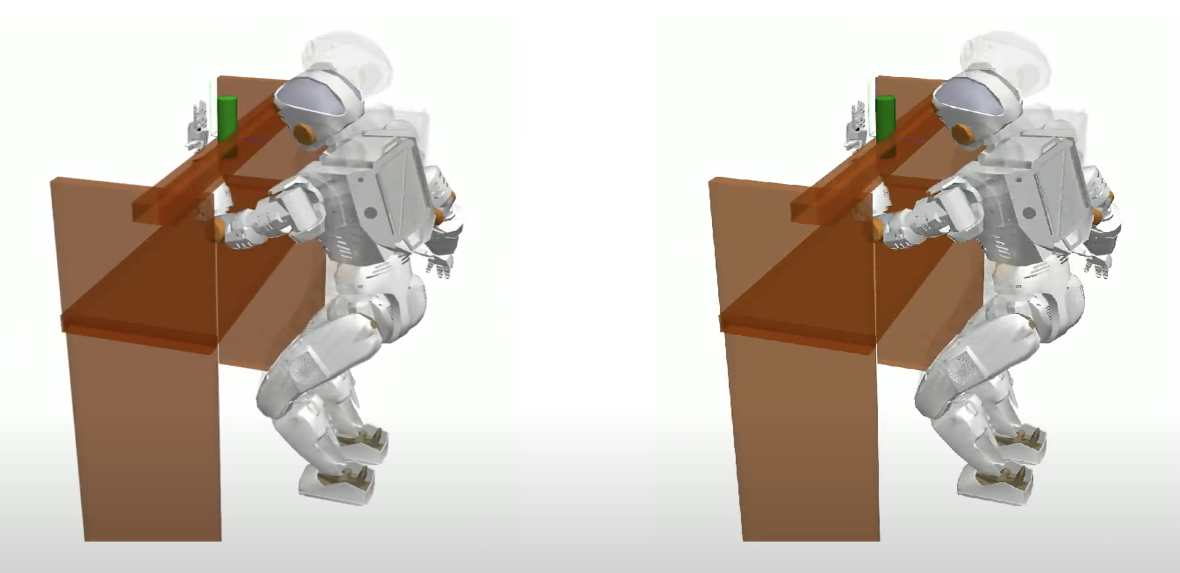
\includegraphics[scale=0.3]{images/motion-planning.png}\hfill
    \caption{Sampling based motion planning of NASA Valkyrie \cite{Vijayakumar}}\hfill
    \label{motion-planning}
\end{figure}

\begin{enumerate}
    \item \textit{Deterministic algorithms -} The deterministic algorithms are developed such that it computes the valid path everytime knowing almost
    all the variables of the environment. Methods such as \textit{cellular decomposition, Voronoi diagrams, visibility graphs, potential fields and Canny's algorithms}
    rely on
    mathematical construction of the environment with the obstacles and provide $\mathit{CS_{obs}}$. Although these algorithms are complete, the computation
    of high-dimensional space is expensive and the environments are always not deterministic.

    \item \textit{Sampling based algorithms -} These algorithms mostly approximate the connectivity of $\mathit{CS_{free}}$ through random sampling configurations
    from $\mathit{CS}$ and rejecting the configurations using boolean collision detection techniques. The main examples are  \textit{Probabilistic Maps and
    Rapidly-exploring Random Trees(RRT)} in combination with Voronoi diagrams promotes the obstacle avoidance configurations for a robot. The main advantage of
    sampling based algorithms are to handle the higher dimensional configuration space recovering a higher degree of completeness.

    \item \textit{Path optimization algorithms -} These algorithms provide optimization in terms of path planning and trajectory planning starting from a valid
    initial state to its goal position with the desired configurations. \textit{Greedy optimization} tries to directly connect the start configuration to 
    its goal state that generates a collision free shortest path by discretizing the path into \textit{n} closest goal configuration relative to previous 
    configuration.
\end{enumerate}

\subsubsection{Motion Planning in Humanoid robots}

Classical motion planning techniques determine collision free trajectories considering only the geometric model of the robot. However the control of
polyarticulated system needs the synthesis of robot models that describe the effect of joint variations on the whole robot configuration. In both the case,
for instance considering an arm moving to it's goal position, the robot tends to make it more unusual, inefficient and unnatural movements. To overcome these 
problems, geometric models are replaced with kinematic models, dynamic models or optimal control and trajectories are generated. Additional constraints like
multiple contacts and dynamic balance of the system are considered. For instance, motion primitives that have been predefined by a human expert based on prior
knowledge can be used to guide the planner \cite{zhang2014motion}. 

~

In case of humanoid walking, the planner can be generated using deterministic approaches with dynamic alterations of the foot transition model considering
the smooth transition of the trajectories for posture transitions. For these cases, sampling-based algorithms are considered to improve the degree of completeness.
Either way, the higher dimensional configuration space is handled so that the problem is solved successively. An example is presented in \cite{yoshida2008planning} where a 36 degree of freedom
robot is reduced to a 3 degrees of freedom bounding box and a PRM is applied for the path planning problem of the box. Another example is to present the
constraints in the form of sub-manifolds of \textit{CS} where a union of separate manifolds like contact limb position and static balance constraints can be 
used to plan the configuration space. In such cases, static balance control in humanoid robots and other legged robots can be obtained \cite{hauser2010multi}.

\subsection{Kinematics Approach}

Generally, \textit{kinematics} is defined as a branch of science which deals with the study of the position, velocity and acceleration of a mechanical system without
considering forces and the dynamic properties of the system (such as mass or inertia) that generate the motion. In humanoid and manipulator robots, the system is 
represented as rigid bodies composed of actuators and sensors. In contrast with the manipulators, the humanoid robots are not fixed to any environment and are highly mobile.
This makes the humanoids (or humanoid robots) more redundant than the manipulators. This section briefs the state of the art and concepts of kinematic approach used in
humanoid control.

\subsubsection{Basic Concepts}

The \textit{joint space} is also called as \textit{configuration space}, of a robot with $n$ degrees of freedom (DoF) is a \textit{n}-dimensional manifold $\mathit{Q}$ containing 
all the possible joint values for a joint $q$ can take. For humanoid robots, this space can be generalized to the operational points \cite{khatib1987unified}, which can represent any part of the body
that may be of interest. In robotics, there exists four subdomains of kinematics namely,  \textit{\textit{(i)} forward kinematics (or direct geometry), \textit{(ii)} inverse kinematics
(or inverse geometry), \textit{(iii)} forward differential kinematics (or simply forward kinematics), and \textit{(iv)} inverse differential kinematics (or simply inverse kinematics).}

\begin{itemize}
    \item \textbf{Direct Geometric Model:} For a robot with $n$ DoF in a $n$-dimensional joint space such that $q \in Q$, there exist a pose $x \in \mathit{SE(3)}$ represented as
    $$x = f(q)$$ described by a map $f:Q \rightarrow \mathit{SE(3)}$.
    
    \item \textbf{Inverse Geometric Model:} For a robot with $n$ DoF in a $n$-dimensional joint space with $q \in Q, x \in \mathit{SE(3)}$, the joint space can be represented from 
    a given pose for a certain operational point as $$q = f^{-1}(x)$$ described by a map $f: \mathit{SE(3) \rightarrow Q}$. But there is a possibility for non-unique solution or 
    non-existing solution (known as singularity).

    \item \textbf{Forward Kinematic Model:} For a robot with $n$ DoF in a $n$-dimensional joint space such that $q \in Q, x \in \mathit{SE(3)}$, the operational twist $\xi \in
     \mathit{SE(3)}$ due to the joint variation $\dot{q}$ is described as $$\xi = J(q)\dot{q}$$ Here, $J$ is the basic Jacobian such that $J : T_q(Q)$ where $T_q(Q)$ is the tangent 
     space of the $Q$ space. Instead, the Jacobian $J$ can be formulated analytically using the pose variation $\dot{x}$ and joint variation $\dot{q}$ as $$\dot{x} = \frac{\partial x}{\partial 
     q}\dot{q} \quad \mathnormal{or} \quad \dot{x} = J\dot{q}$$ then $J$ is the task Jacobian.

     \item \textbf{Inverse Kinematic Model:} For a robot with $n$ DoF in a $n$-dimensional joint space such that $q \in Q, x \in \mathit{SE(3)}$, finding the joint variations $\dot{q}$
     that produce a pose variation $\dot{x}$ of the end effector as $$\dot{q} = J^{-1} \dot{x}$$ and it can be solved iteratively.
\end{itemize}

\subsubsection{Kinematics Approach in humanoid robots}


\subsection{Dynamics Approach}
\subsection{Optimal Control}

\section{Approaches in Humanoid Balance Control}
\subsection{Linear Inverse Pendulum Approach}


Consider a simple inverted pendulum model as in figure [\ref{ipm}] with mass $m$ and link length $l_1$, the kinematics and dynamics for the model can be represented as,

\begin{figure}[h!]
    \centering
    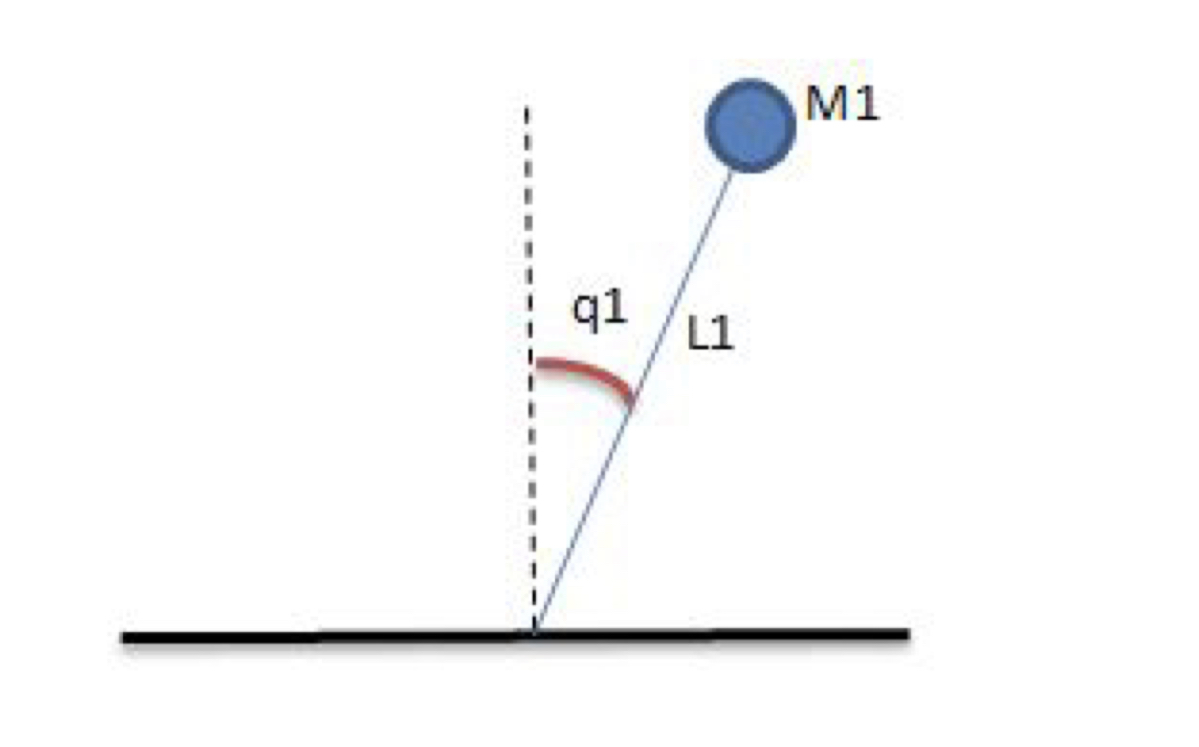
\includegraphics[scale=.15]{images/ipm.jpeg}\hfill
    \caption{Simple Inverse Pendulum Model}\hfill
    \label{ipm}
\end{figure}

Position:
\begin{equation}
\begin{split}
    x_1 &= -l_1\sin{q_1} \\
    y_1 &= l_1\cos{q_1}
\end{split}
\end{equation}

Velocity:
\begin{equation}
\begin{split}
    \Dot{x_1} &= -l_1\cos({q_1})\Dot{q_1} \\
    \Dot{y_1} &= -l_1\sin({q_1})\Dot{q_1}
\end{split}
\end{equation}

Acceleration:
\begin{equation}
\begin{split}
    \Ddot{x_1} &= l_1 \sin{(q_1)}\Dot{q_1}^2 - l_1\cos{(q_1)}\Ddot{q_1} \\
    \Ddot{y_1} &= -l_1 \cos{(q_1)}\Dot{q_1}^2 - l_1 \sin{(q_1)}\Ddot{q_1}
\end{split}
\end{equation}

Forces and Torques:
\begin{equation}
\begin{split}
    m_1\Ddot{x_1} &= F_{x1} \\
    m_1\Ddot{y_1} &= F_{y1} - m_1g
\end{split} 
\end{equation}
\begin{equation}
    \tau_1 = m_1l_1^2\Ddot{q_1} + m_1gl_1\sin{q_1}
\end{equation}

where $F_{x1}$ and $F_{y1}$ represent the reaction forces on the link from the fixed point.

\subsection{Double Inverse Pendulum Approach}

Consider a double inverted pendulum model as in figure [\ref{dipm}] with mass $m$ and link lengths $l_1$ and $l_2$, the kinematics and dynamics for the model can be represented as,

\begin{figure}[h!]
    \centering
    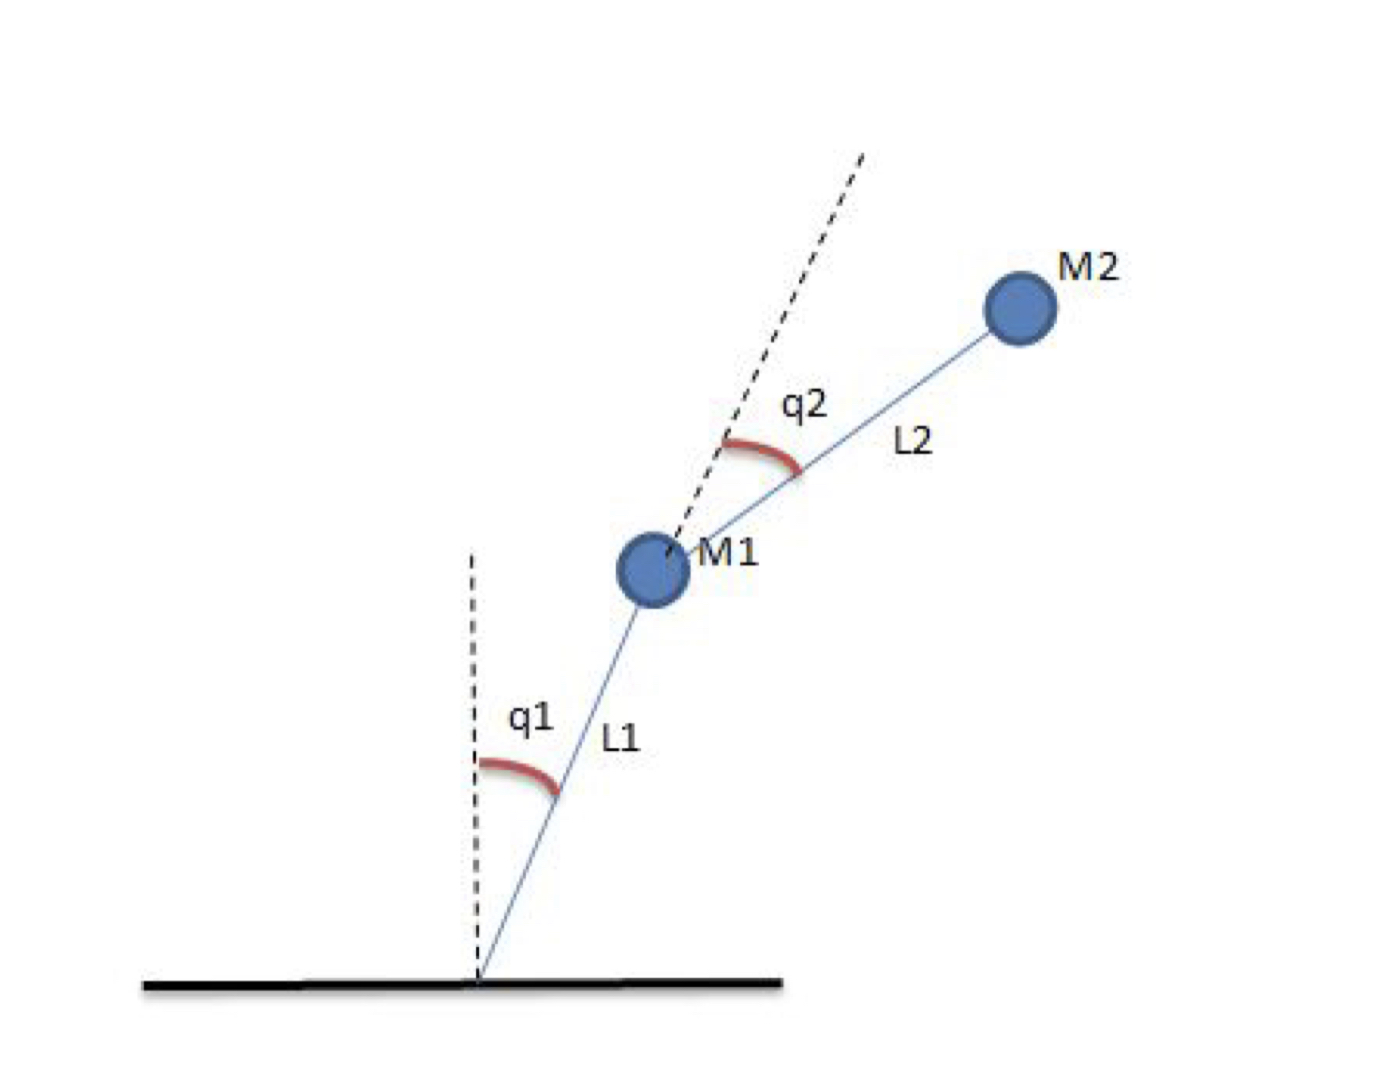
\includegraphics[scale=0.15]{images/dipm.jpeg}\hfill
    \caption{Double Inverse Pendulum Model}\hfill
    \label{dipm}
\end{figure}

Position:
\begin{equation}
\begin{split}
    x_1 &= -l_1\sin{q_1} \\
    y_1 &= l_1\cos{q_1}
\end{split}
\end{equation}

\begin{equation}
\begin{split}
    x_2 &= -l_1\sin{q_1} - l_2\sin{(q_1+q_2)} \\
    y_2 &= l_1\cos{q_1} + l_2\cos{(q_1+q_2)}
\end{split}
\end{equation}

Velocity:
\begin{equation}
\begin{split}
    \Dot{x_1} &= -l_1\cos(q_1)\Dot{q_1} \\
    \Dot{y_1} &= -l_1\sin(q_1)\Dot{q_1}
\end{split}
\end{equation}

\begin{equation}
\begin{split}
    \Dot{x_2} &= -l_1\cos(q_1)\Dot{q_1} - -l_1\cos(q_1+q_2)\Dot{(q_1+q_2)} \\
    \Dot{y_2} &= -l_1\sin(q_1)\Dot{q_1} - -l_1\sin(q_1+q_2)\Dot{(q_1+q_2)}
\end{split}
\end{equation}

Acceleration:
\begin{equation}
\begin{split}
    \Ddot{x_1} &= l_1 \sin{(q_1)}\Dot{q_1}^2 - l_1 \cos{(q_1)}\Ddot{q_1} \\
    \Ddot{y_1} &= -l_1 \cos{(q_1)}\Dot{q_1}^2 - l_1 \sin{(q_1)}\Ddot{q_1}
\end{split}
\end{equation}

\begin{equation}
\begin{split}
    \Ddot{x_2} &= -l_1\cos{(q_1)}\Ddot{q_1} + l_1\sin{(q_1)}\Dot{q_1}^2 - l_2\cos{(q_1+q_2)}(\Ddot{q_1} + \Ddot{q_2}) + l_2\sin(q_1+q_2)(\Dot{q_1} + \Dot{q_2})^2 \\
    \Ddot{y_2} &= -l_1\sin{(q_1)}\Ddot{q_1} + l_1\sin{(q_1)}\Dot{q_1}^2 - l_2\sin{(q_1+q_2)}(\Ddot{q_1} + \Ddot{q_2}) + l_2\cos(q_1+q_2)(\Dot{q_1} + \Dot{q_2})^2
\end{split}
\end{equation}

Forces and Torques:
\begin{equation}
\begin{split}
    m_1\Ddot{x_1} &= F_{x1} + F_{x_2} \\
    m_1\Ddot{y_1} &= F_{y1} + F_{y_2} - m_1g
\end{split}
\end{equation}

\begin{equation}
\begin{split}
    m_2\Ddot{x_2} &= F_{x2} \\
    m_2\Ddot{y_2} &= F_{y2} - m_2g
\end{split}
\end{equation}

where $F_{x1}$,$F_{x2}$,$F_{x3}$ and $F_{y1}$,$F_{y2}$,$F_{y3}$ represent the reaction forces on the link from the fixed point.

\begin{equation}
\begin{split}
    \tau_1 &= m_1l_1^2\Ddot{q_1} + m_1gl_1\sin{q_1} \\
    \tau_2 &= m_2l_2^2 (\Ddot{q_1} + \Ddot{q_2}) + m_2gl_2\sin(q_1+q_2)
\end{split}
\end{equation}

\subsection{Cart Table Model}
\subsection{Spherical Inverse Pendulum Approach}

\section{Approaches in Posture Control and Motion Retargetting}
\subsection{Mansard's work}
\subsection{D. Gucci's work}
\subsection{Kumar Munirathinam's work}

